\section{Durchführung}
\label{sec:Durchführung}

Die Durchführung des Experiments wird aus drei Teilen bestehen, die im Folgenden 
erläutert werden. Zunächst befindet sich der Hauptbestandteil in \autoref{fig:4} 
\begin{figure}[H]
    \centering
        \centering
        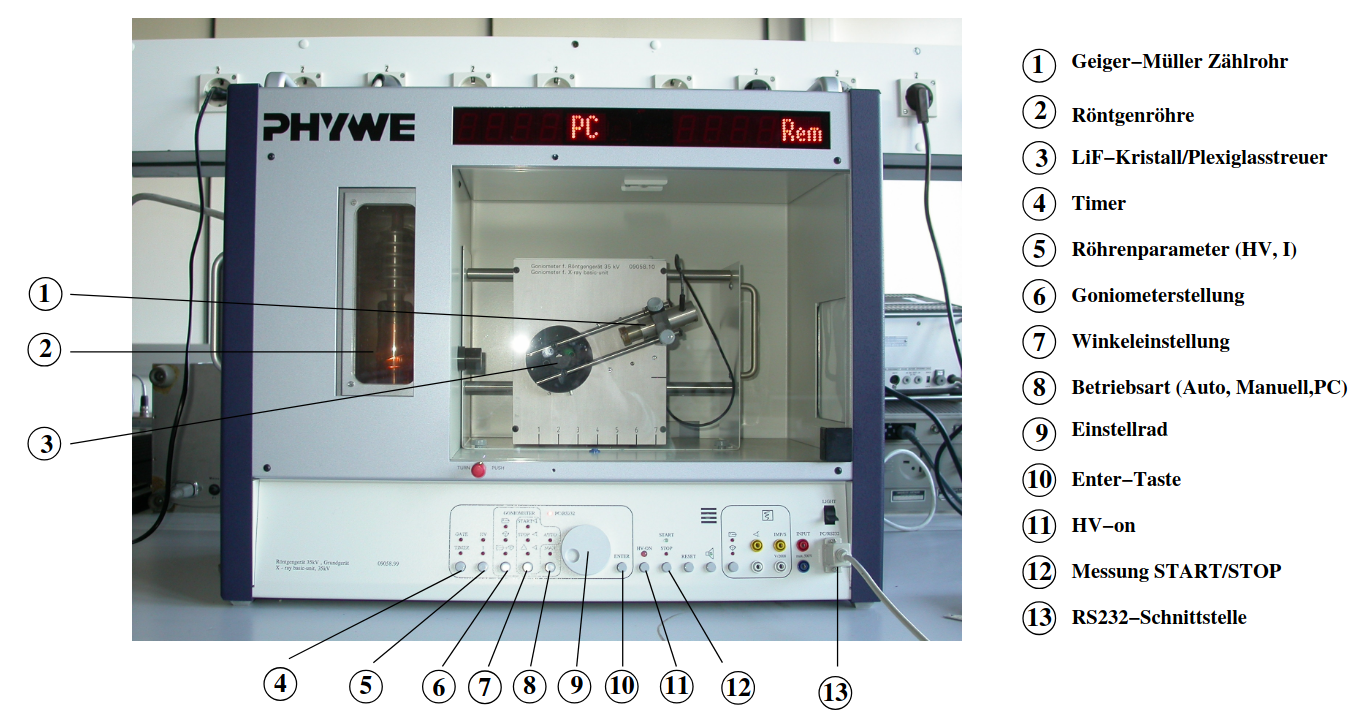
\includegraphics[width=\textwidth]{bilder/roehre.png}
        \caption{Röntgengerät mit Komponenten. \cite{anleitung10}}
    \hfill
    \label{fig:4}
\end{figure}
\noindent Mittig befinden sich das Geiger-Müller-Zählrohr, welches mit verschiedenen 
Aufsätzen der zu untersuchenden Proben versehen werden kann, die Röntgenröhre und 
der Kristall. Neben abgebildeten der Apparatur ist auch ein Computer zur
Verarbeitung der Daten Bestandteil des Versuchs. Dieser ist zuständig für die
Start- und Endwinkel des Kristalls, die Integrationszeit und die Schrittweite.
Für die Bewegung der Instrumente könnte der Kistallwinkel fixiert eingestellt 
werden, sodass nur das Zählrohr die Winkel abläuft. Andererseits wäre auch der 
2:1-Kopplungsmodus eine Möglichkeit, bei dem sich Zählrohr mit dem doppelten 
Winkel des Kristalls bewegt. In diesem Versuch wird sich auf letzteres beschränkt. 
\vspace{0.5em}
\\
\noindent Als Einstellungen werden eine konstante Beschleunigungsspannung von 
$U = 35 \unit{\kilo\volt}$ und ein Emissionsstrom von $I = 1 \unit{\milli\ampere}$
gewählt, die über den gesamten Versuch nicht variiert werden.

\subsection{Emissionsspektrum einer Kupfer-Röntgenröhre}
Für das Emissionsspektrum der Cu-Röntgenröhre wird bei einer Beugungsordnung von 
$n = 1$ im Winkelbereich von 4° bis 26° in 0.26°-Schritten die Zählrate gemessen.
die Integrationszeit pro Winkel liegt bei $\increment t = 5 \unit{seconds}$.

\subsection{Absorptionsspektrum verschiedener Materialien}
In diesem Bereich sollen die Absorptionsspektren von Gallium, Brom, Strontium, 
Zink und Zirkonium untersucht werden. Dazu werden Absorber mit den Proben 
vor dem Geiger-Müller-Zählrohr befestigt und in einem Winkel von $\pm 1°$ von 
dem materialabhängigen Bragg-Winkel $\theta_K^{Lit}$ gemessen. Dieses Mal 
beträgt die Messzeit 20 Sekunden bei einem Winkelzuwachs von 0.1°.

\subsection{Verifizierung der Bragg-Reflexion}
Für die Überprüfung der Bragg-Bedingung wird der LiF-Kristall auf 14° fixiert.
Das Zählrohr soll die Zählrate in einem Bereich 26° bis 30°, erneut bei einer 
Schrittweite von 0.1°. Die Integrationszeit wird wieder zurück auf 
$\increment t = 5 \unit{seconds}$ gesetzt.